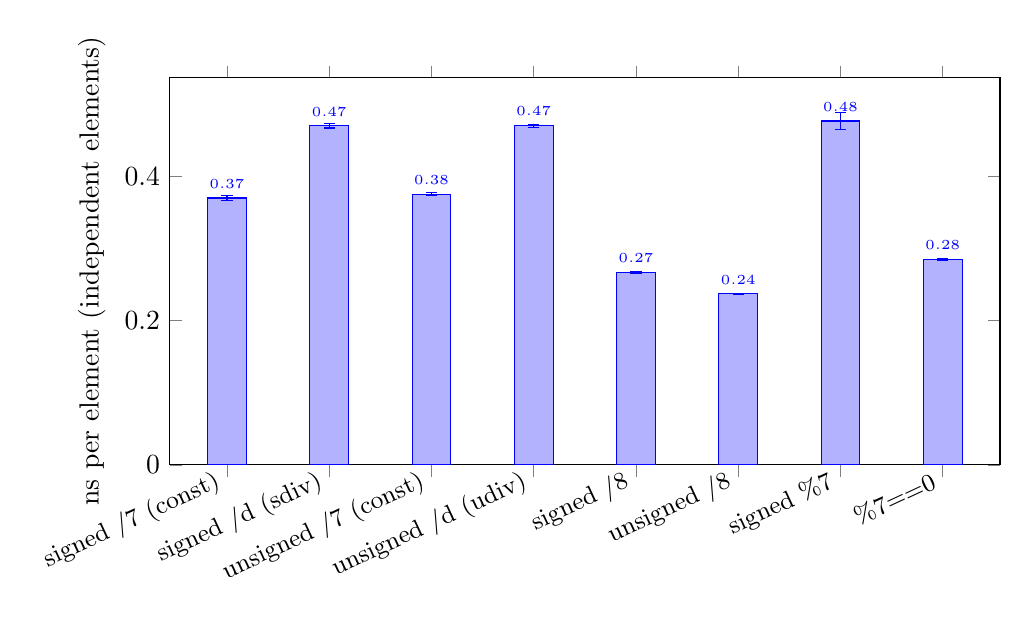
\begin{tikzpicture}
\begin{axis}[ybar, width=\textwidth, height=6.5cm, bar width=14pt, ymin=0, symbolic x coords={signed /7 (const),signed /d (sdiv),unsigned /7 (const),unsigned /d (udiv),signed /8,unsigned /8,signed \%7,\%7==0}, xtick=data, x tick label style={rotate=25, anchor=east, font=\small}, ylabel={ns per element (independent elements)}, enlarge x limits=0.08, legend style={font=\small, at={(0.98,0.98)}, anchor=north east}, nodes near coords, nodes near coords style={font=\tiny}, every node near coord/.append style={/pgf/number format/.cd, fixed, precision=2}]
\addplot+[error bars/.cd, y dir=both, y explicit] coordinates {(signed /7 (const),0.3698) +- (0,0.0037) (signed /d (sdiv),0.4696) +- (0,0.0029) (unsigned /7 (const),0.3751) +- (0,0.0023) (unsigned /d (udiv),0.4699) +- (0,0.0021) (signed /8,0.2662) +- (0,0.0013) (unsigned /8,0.2370) +- (0,0.0010) (signed \%7,0.4764) +- (0,0.0115) (\%7==0,0.2845) +- (0,0.0012)};
\end{axis}
\end{tikzpicture}